
\documentclass{IOS-Book-Article}

\usepackage{mathptmx}
\usepackage{soul}\setuldepth{article}
\usepackage{graphicx}
\graphicspath{ {./figures/} }
%\usepackage{times}
%\normalfont
%\usepackage[T1]{fontenc}
%\usepackage[mtplusscr,mtbold]{mathtime}
%
\def\hb{\hbox to 11.5 cm{}}

\begin{document}

\pagestyle{headings}
\def\thepage{}
\begin{frontmatter}              % The preamble begins here.


%\pretitle{Pretitle}
\title{First Steps towards a Risk of Bias Corpus of Randomized Controlled Trials}

\markboth{}{April 2022\hb}
%\subtitle{Subtitle}

\author[A,B]{\fnms{Anjani} \snm{Dhrangadhariya}\orcid{0000-0003-1691-1338}%
\thanks{Corresponding Author: Anjani Dhrangadhariya, University of Applied Sciences Western Switzerland (HES-SO), Technopole 3,
3960 Sierre, Switzerland; E-mail:
anjani.dhrangadhariya@hevs.ch.}},
\author[C,D]{\fnms{Roger} \snm{Hilfiker}}
,
\author[C,D]{\fnms{Martin} \snm{Sattlemayer}}
,
\author[C,D]{\fnms{Katia} \snm{Giacomino}}
,
\author[C,D]{\fnms{Rahel} \snm{Caliesch}}
,
\author[C,D]{\fnms{Simone} \snm{Elsig}}
,
\author[E,F]{\fnms{Nona} \snm{Naderi}}
and
\author[A,B]{\fnms{Henning} \snm{M\"uller}}

\runningauthor{A. Dhrangadhariya et al.}
\address[A]{Informatics Institute, HES-SO Valais-Wallis, Sierre, Switzerland}
\address[B]{University of Geneva (UNIGE), Geneva, Switzerland}
\address[C]{School of Health Sciences, HES-SO Valais-Wallis, Leukerbad, Switzerland.}
\address[D]{Department of Physiotherapy, HES-SO Valais-Wallis, Leukerbad, Switzerland.}
\address[E]{Geneva School of Business Administration, HES-SO Geneva, Switzerland.}
\address[F]{SIB Swiss Institute of Bioinformatics (SIB), Geneva, Switzerland}

\begin{abstract}
Risk of bias (RoB) assessment of randomized clinical trials (RCTs) is vital to conducting systematic reviews. 
Manual RoB assessment for hundreds of clinical trials is a cognitively demanding, lengthy process and is prone to subjective judgment. 
Supervised machine learning (ML) can help to accelerate this process but requires a hand-labelled corpus.
There are currently no RoB annotation guidelines or any annotated corpus.
In this pilot annotation project, we test the feasibility of directly using the revised Cochrane RoB 2.0 tool for RCTs for developing an RoB annotated corpus. 
We also test a multi-level annotation scheme for annotating RCTs with RoB categories.
We report inter-annotator agreement among four experienced annotators, which ranges between 0\% for some RoB classes and 76\% for others.
Finally, we discuss the shortcomings of this direct translation of annotation guidelines and scheme and suggest approaches to improve them to obtain an RoB annotated corpus suitable for ML.
\end{abstract}

\begin{keyword}
risk of bias\sep annotation\sep
systematic reviews\sep corpus\sep automation
\end{keyword}
\end{frontmatter}
\markboth{April 2022\hb}{April 2022\hb}
%\thispagestyle{empty}
%\pagestyle{empty}
%
%
%
\section{Introduction}
\label{sec:intro}
%
Systematic reviews (SRs) synthesized from randomized controlled trials (RCTs) are the highest quality of evidence in the evidence hierarchy.
In theory, an RCT accurately measures the treatment effect on patient outcomes but can be biased in practice due to flawed study design, execution, analysis or outcome reporting.\cite{hariton2018randomised}
Biases in RCTs cannot be measured, but the risk of bias (RoB) can be assessed.
The researchers conducting SRs must rigorously look for possible biases before incorporating them into SRs.
Published RCTs are exponentially increasing~\footnote{\url{https://pubmed.ncbi.nlm.nih.gov/?term=randomized\%20controlled\%20trial&filter=pubt.randomizedcontrolledtrial}} over time, so manual RoB assessment for every study becomes a protracted process.
Machine learning (ML) can help accelerate this process by directly pointing the reviewers to the parts of the text relevant to identifying RoB, leading to quickly judging the trial quality.
Both Marshall \textit{et al.} and Millard \textit{et al.} attempted RoB assessment, albeit using proprietary, paywalled data~\cite{marshall2015automating,millard2016machine}.
Recently, Wang \textit{et al.} released a hand-labelled RoB corpus for animal studies using a preclinical RoB assessment tool.~\cite{wang2022risk}.
However, to date, we neither know any publicly available hand-labelled corpus for human RCTs using the widely used revised Cochrane's RoB 2.0 tool (RoB 2.0) nor any corpus annotation guidelines that could help to annotate one.~\cite{sterne2019rob,lansbury2020co}
RoB assessment is a knowledge-heavy task where even highly trained experts are prone to subjective judgments.
The primary requirement to develop such a corpus entails creating a clear-cut annotation scheme and guidelines, and as neither of them exists, this work is focused on two primary concerns.
1) To test whether RoB 2.0 tool could be used as RoB corpus annotation guidelines to develop a corpus that could be used for training supervised ML models.
2) To develop and test an RoB annotation scheme that closely mimics the RoB 2.0 tool.~\cite{sterne2019rob}
%
%
%
\section{Methods}
\label{sec:methods}
%
\subsection{Formulating Annotation Scheme}
%
We formulate the annotation scheme as a function of the RoB 2.0 tool.
The tool divides biases into five risk domains which further decompose into several signalling questions, each corresponding to different parts of the trial design.
Each signalling question prompts the reviewer to look for a piece(s) of factual evidence in the clinical study to respond with one of the five response options: ``Yes'', ``Probably yes'', ``No'', ``Probably no'', or ``No information''.
E.g. to respond to the signalling question ``Was the allocation sequence random?'', the reviewers need to identify whether a proper methodology was used for participant allocation and only if a proper methodology is identified the reviewer responds to this question as ``Yes'' and otherwise ``No''.

We formulate an annotation scheme where each signalling question is an entity.
Each entity has five entity labels corresponding to the five response options to that question.
Entities aim to represent the factual evidence from the RCTs, and the entity labels aim to incorporate the reviewer's risk judgment for the identified evidence.
The cumulative risk judgment from each risk domain could be estimated using decision flowcharts combining the responses from all the signalling questions.
The flowchart allows this risk judgment to be classified as either ``Low-risk'', ``High-risk'' or ``Some-concerns'' (refer the Figure~\ref{fig:flowchart}).
To account for this, we have an additional document-level annotation scheme for each risk domain whereby a reviewer can choose either of the three risk judgments.
%
%
%
\section{Results}
\label{sec:results}
%
%Therefore, each entity could have one of the five response options incorporating the reviewer's judgment of the answer.
%The reviewer needs to mark the identified text evidence (a phrase, sentence (s), or paragraph) with the RoB entity along with one of the five response options.
%We have a hierarchical annotation scheme comprising 22 entities corresponding to the 22 signalling questions, each with five response options.


A visual representation of our annotation scheme is illustrated in Figure~\ref{fig:ann_scheme}. 
%
\begin{figure}[ht]
    \centering
    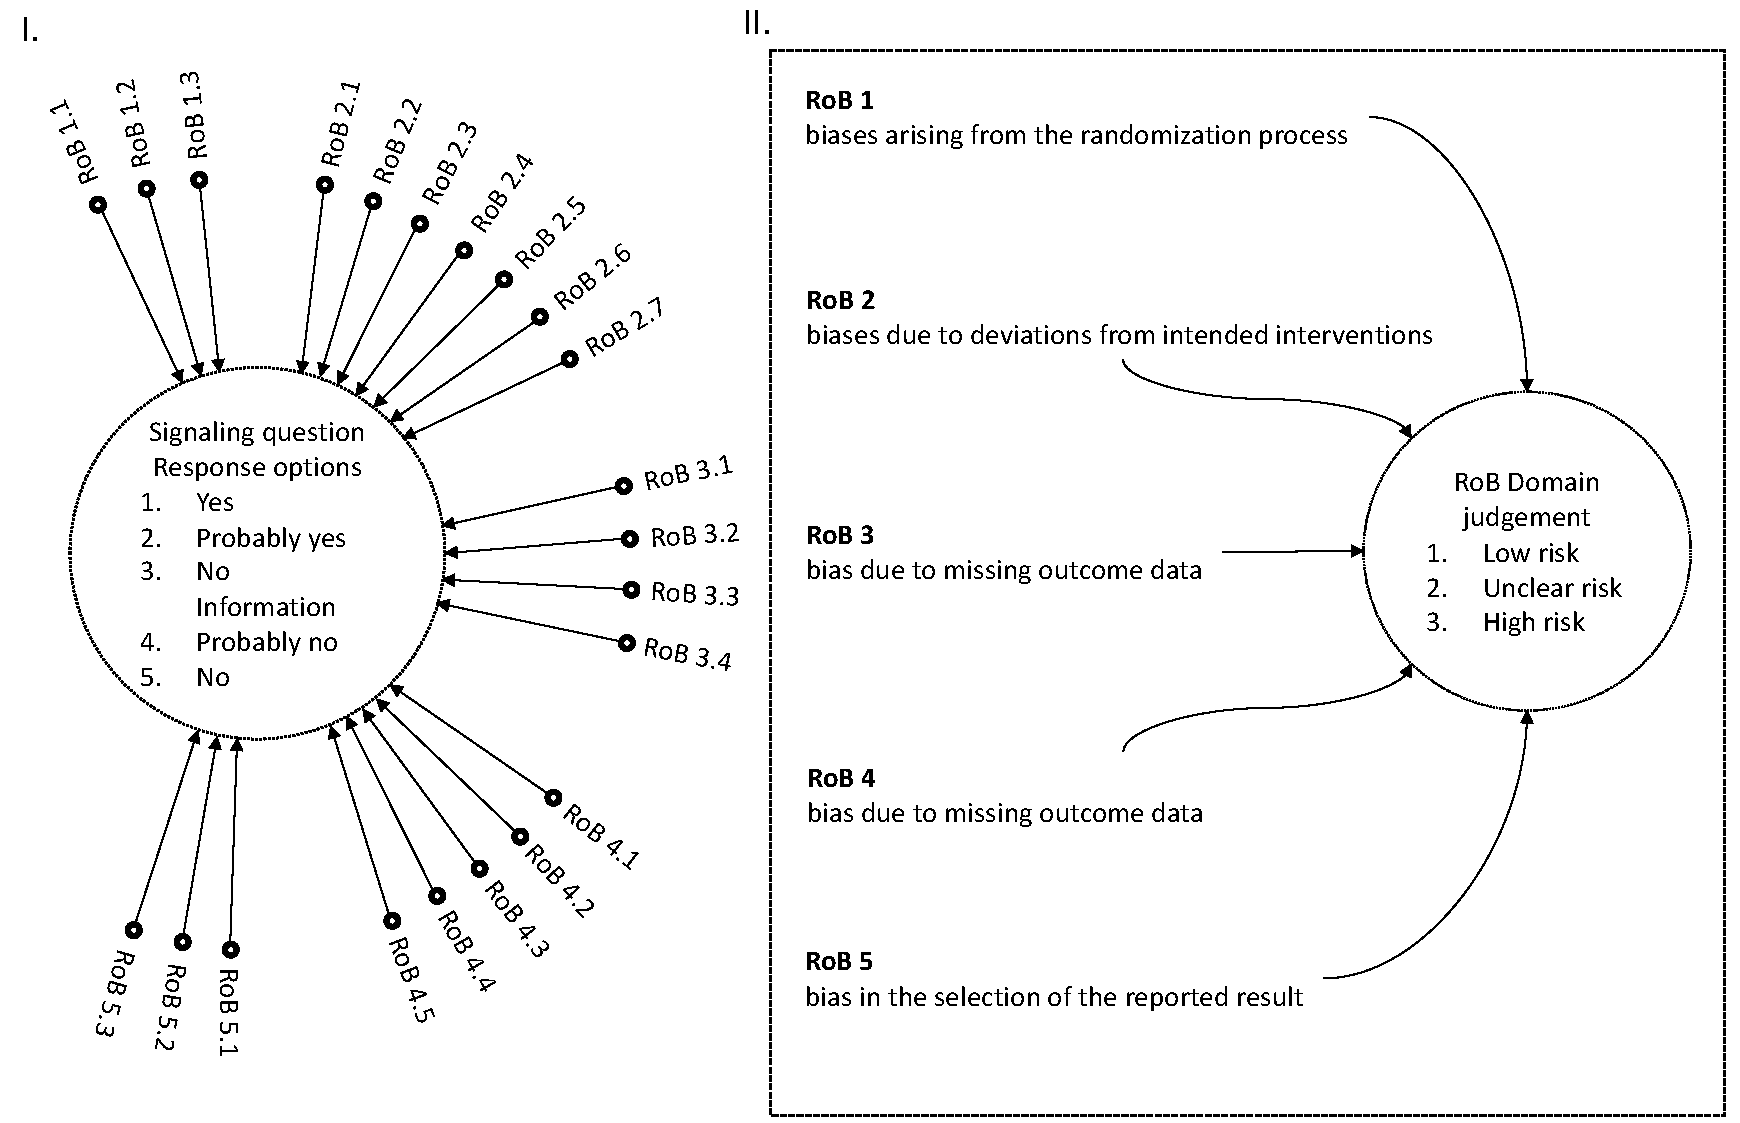
\includegraphics[width=0.70\textwidth]{Figures/figures2.pdf}
    \caption{Annotation scheme. I. signalling question annotation scheme: each signalling question (RoB 1.1, 1.2, 1.3, 2.1, ...) is an entity/class that could take either of five response options or attributes. II. Risk domain annotation scheme: each risk domain (RoB 1, 2, 3, 4, and 5) is a class that could take either of three risk classes based on the assessment of RoB signalling questions. This final risk domain judgment depends upon instructions from RoB 2.0 guidelines.}
    \label{fig:ann_scheme}
\end{figure}
%
%
%
\section{Discussion}

\section{Conclusion}
\label{sec:conclusion}
%
In conclusion, revised Cochrane's RoB assessment 2.0 tool cannot be directly used as RoB corpus annotation guidelines.
The annotation scheme directly adapted from RoB 2.0 document also needs improvement, as detailed in the discussion section.
The annotation scheme directly adapted from RoB 2.0 document also needs improvement, as detailed in the discussion section.
We are using insights gained this pilot project to develop crisp annotation guidelines to obtain consistent annotations.
The annotated RCTs from this study are available on Zenodo (DOI: ).
%
%
%
%%%%% References %%%%%
\bibliographystyle{spiebib} 
%
%
\bibliography{bibliography}
%
\end{document}
